\documentclass[11pt]{article}

\usepackage[utf8]{inputenc}
\usepackage{amsmath, amssymb}
\usepackage{graphicx}
\usepackage{cite}
\usepackage{geometry}
\usepackage{float}
\usepackage{booktabs}
\usepackage{hyperref}
\geometry{margin=1in}

\graphicspath{{figures/}}

\title{\textbf{Characterization of Radiation-Induced Defects in FeNiCrCoCu
High-Entropy Alloy Using SOAP-Based Methods}}

\author{
S. Bergamin$^{1}$, E. Bringa$^{1}$ \\[4pt]
$^{1}$[Completar afiliación institucional]
}

\date{}

\begin{document}

\maketitle

\begin{abstract}
Understanding radiation damage in complex alloys is critical for the development
of next-generation nuclear materials. In this work, we analyze defect formation
in a FeNiCrCoCu high-entropy alloy subjected to a thermal spike using both
classical Wigner--Seitz analysis and modern descriptor-based methods. In
particular, we employ the Smooth Overlap of Atomic Positions (SOAP) descriptor
to identify distorted atomic environments and detect vacancy regions without
relying on a reference lattice. A total of $20{,}629$ atoms ($\approx 2\%$ of
the system) were classified as distorted using a distance threshold of
$d^i \geq 0.15$. Descriptor-space analysis via PCA reveals clear separation
between lattice and defect populations. Our results highlight the limitations
of traditional approaches at high temperature and demonstrate the robustness of
descriptor-based methodologies.
\end{abstract}

% ─────────────────────────────────────────────────────────────────────────────
\section{Introduction}
% ─────────────────────────────────────────────────────────────────────────────

The development of materials capable of withstanding extreme radiation
environments is a central challenge in nuclear science. Energetic particles
deposit energy through nuclear and electronic stopping, generating collision
cascades and thermal spikes that produce Frenkel pairs and defect clusters
\cite{Was2017, Zinkle2009}.

High-entropy alloys (HEAs) have emerged as promising candidates due to their
enhanced radiation tolerance and sluggish diffusion effects
\cite{Yeh2004, Cantor2004, Zhang2015radiation, Granberg2016}. Among them,
FeNiCrCoCu is a prototypical FCC alloy widely studied for radiation resistance.

Traditional defect identification methods such as Wigner--Seitz (WS) analysis
rely on a reference lattice and lose accuracy at high temperature.
Descriptor-based approaches such as SOAP provide a robust alternative by
encoding local atomic environments into high-dimensional vectors
\cite{Bartok2013}.

In this work, we apply a SOAP-based pipeline inspired by the FaVaD framework
to characterize radiation-induced defects and compare results with classical WS
analysis.

% ─────────────────────────────────────────────────────────────────────────────
\section{Methodology}
% ─────────────────────────────────────────────────────────────────────────────

\subsection{Simulation Setup}

The system consists of $1{,}024{,}000$ atoms arranged in an FCC FeNiCrCoCu
structure with periodic boundary conditions. Radiation damage was introduced
by a cylindrical thermal spike of $2$\,nm diameter with an initial temperature
of $50{,}000$\,K. The system was allowed to cool and the configuration at
timestep $160{,}000$ was analyzed.

[COMPLETAR: potencial interatómico, timestep, temperatura inicial]

\subsection{Wigner--Seitz Analysis}

The damaged structure was analyzed using the Wigner--Seitz method implemented
in OVITO. Vacancies correspond to empty lattice sites, while interstitials
correspond to double occupancy. A total of $3{,}867$ vacancies and $3{,}669$
interstitials were identified.

\subsection{SOAP Descriptor}

Each atomic environment was encoded using the SOAP descriptor:

\begin{equation}
p^i_{nn'l} = \pi\sqrt{\frac{8}{2l+1}} \sum_{m=-l}^{l} c^i_{nlm}\,c^i_{n'lm}
\label{eq:soap}
\end{equation}

The descriptor dimension was $D = 450$, using $n_{\max} = 9$,
$l_{\max} = 9$, and $r_{\mathrm{cut}} = 5.0$\,\AA. Each vector was normalized
to unit length.

\subsection{Reference Fingerprint}

The reference fingerprint is defined as the mean descriptor over all atoms in
an unperturbed frame:

\begin{equation}
\bar{q}(T) = \frac{1}{N_{\mathrm{ref}}}
             \sum_{i=1}^{N_{\mathrm{ref}}} \tilde{q}^{\,i}
\label{eq:ref}
\end{equation}

Distances to this reference are computed as:

\begin{equation}
d^i = \left\| \tilde{q}^{\,i} - \bar{q}(T) \right\|_2
\label{eq:dist}
\end{equation}

\subsection{Chi-Distribution Model}

The distribution of SOAP distances in a perfect lattice follows a
chi distribution:

\begin{equation}
P(d \mid k,\sigma) \propto d^{k-2}
\exp\!\left(-\frac{d^2}{2\sigma^2}\right)
\label{eq:chi}
\end{equation}

The best-fit parameters for the present system are $k = 2.0$ and
$\sigma = 0.0315$.  Figure~\ref{fig:hist} shows the full distance
distribution for all $1{,}024{,}000$ atoms together with the classification
threshold. The linear-scale panel reveals the dominant lattice peak, while the
semilogarithmic panel exposes the extended tail of distorted environments.

\begin{figure}[H]
  \centering
  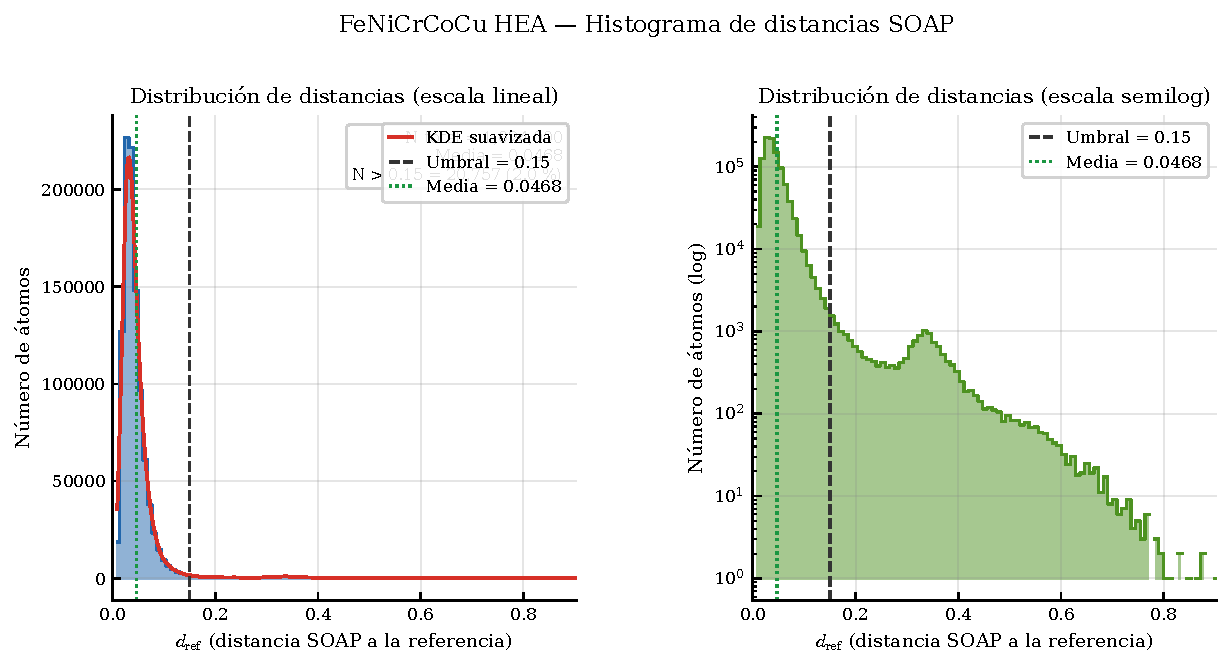
\includegraphics[width=\textwidth]{hist_output_hea_hist}
  \caption{Distribution of SOAP distances $d^i$ (Eq.~\ref{eq:dist}) for all
    $1{,}024{,}000$ atoms of the FeNiCrCoCu HEA after thermal-spike damage.
    \textbf{Left:} linear scale with kernel-density estimate (red curve) and
    the mean distance (dotted green line). The sharp peak near $d^i \approx 0$
    corresponds to atoms in nearly perfect lattice environments.
    \textbf{Right:} semilogarithmic scale revealing the high-distance tail
    ($d^i \geq 0.15$, dashed line) associated with radiation-induced distorted
    environments ($20{,}629$ atoms, $\approx 2.0\%$ of the system).
    Fit parameters: $k = 2.0$, $\sigma = 0.0315$.}
  \label{fig:hist}
\end{figure}

\subsection{Defect Classification}

Atoms with $d^i \geq 0.15$ were classified as distorted (\textit{Unknown}),
yielding $20{,}629$ distorted atoms in total.

\subsection{Grid-Based Vacancy Detection}

Vacancies were also detected using a grid-based method that searches for
regions of low atomic density:

\begin{equation}
\mathcal{V} = \left\{
  \mathbf{g} \;\Big|\;
  \min_{j} \left|\mathbf{g} - \mathbf{r}_j\right| > d_{\mathrm{vac}}
\right\}
\label{eq:grid}
\end{equation}

with $d_{\mathrm{vac}} = 2.0$\,\AA, identifying $252$ vacancy grid points.

% ─────────────────────────────────────────────────────────────────────────────
\section{Results and Discussion}
% ─────────────────────────────────────────────────────────────────────────────

\subsection{SOAP Classification Overview}

Figure~\ref{fig:overview} presents a six-panel overview of the SOAP
classification results. The distance histogram (top left) and violin plot
(center left) confirm that the vast majority of atoms ($1{,}003{,}371$,
$97.99\%$) remain in near-perfect lattice environments
($d^i < 0.15$), while a minority of $20{,}629$ atoms ($2.01\%$) are flagged
as distorted.

The spatial projections (top right, center right) reveal that the distorted
atoms are not uniformly distributed: they cluster along the track of the
thermal spike, consistent with the cylindrical damage morphology introduced
in the simulation. The bar chart (bottom left) summarizes the classification
statistics and confirms that the Unknown population is well separated from
the Lattice background. The \textit{defect\_prob} distribution (bottom right)
shows that distorted atoms tend toward low probability values under the
chi-distribution model, providing an independent probabilistic measure of
anomalous environments.

\begin{figure}[H]
  \centering
  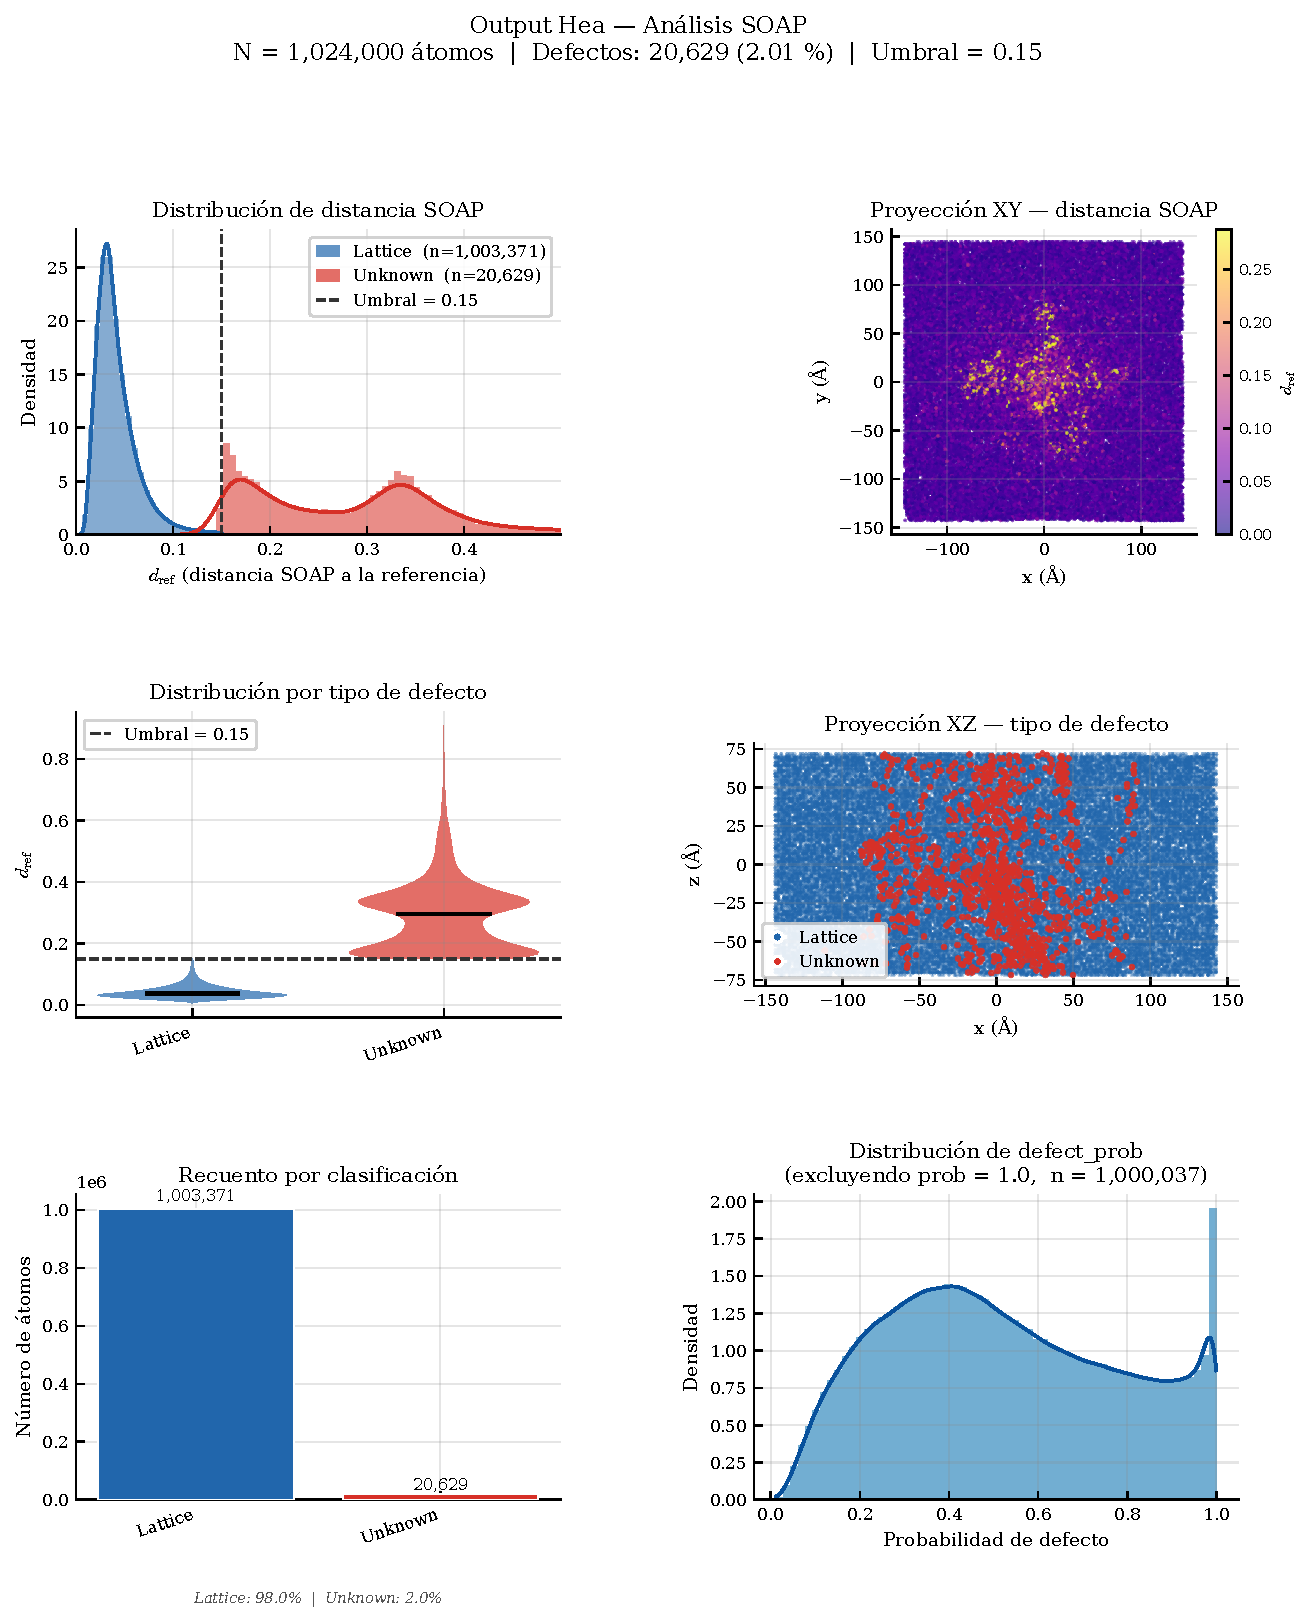
\includegraphics[width=\textwidth]{output_hea_overview}
  \caption{Six-panel classification overview for the FeNiCrCoCu HEA
    ($N = 1{,}024{,}000$ atoms, threshold $d^i = 0.15$).
    \textbf{Top left:} SOAP distance distribution with KDE curves for each
    class (blue = Lattice, red = Unknown) and the classification threshold
    (dashed line).
    \textbf{Top right:} XY spatial projection coloured by $d^i$; the track
    of the thermal spike is visible as a high-distance column.
    \textbf{Centre left:} Violin plot of $d^i$ per class.
    \textbf{Centre right:} XZ spatial projection coloured by defect type.
    \textbf{Bottom left:} Atom counts and percentages per class.
    \textbf{Bottom right:} Distribution of the chi-distribution defect
    probability for atoms with $\text{defect\_prob} < 1$.}
  \label{fig:overview}
\end{figure}

\subsection{Descriptor-Space Analysis}

Figure~\ref{fig:pca} shows the first two principal components of the
SOAP descriptor space. The leftmost panel, coloured by defect type, shows
a compact Lattice cluster (blue) surrounded by a scattered Unknown population
(red), confirming that the descriptor encodes physically meaningful information
about atomic environments. The centre panel, coloured by $d^i$, reproduces
the spatial gradient expected from the chi-distribution model: atoms near the
Lattice cluster have $d^i \approx 0$, while those in the outskirts of the PCA
space carry large distances. The rightmost panel reproduces the distance
histogram in the descriptor-space context, highlighting how the two populations
overlap only marginally near the threshold.

\begin{figure}[H]
  \centering
  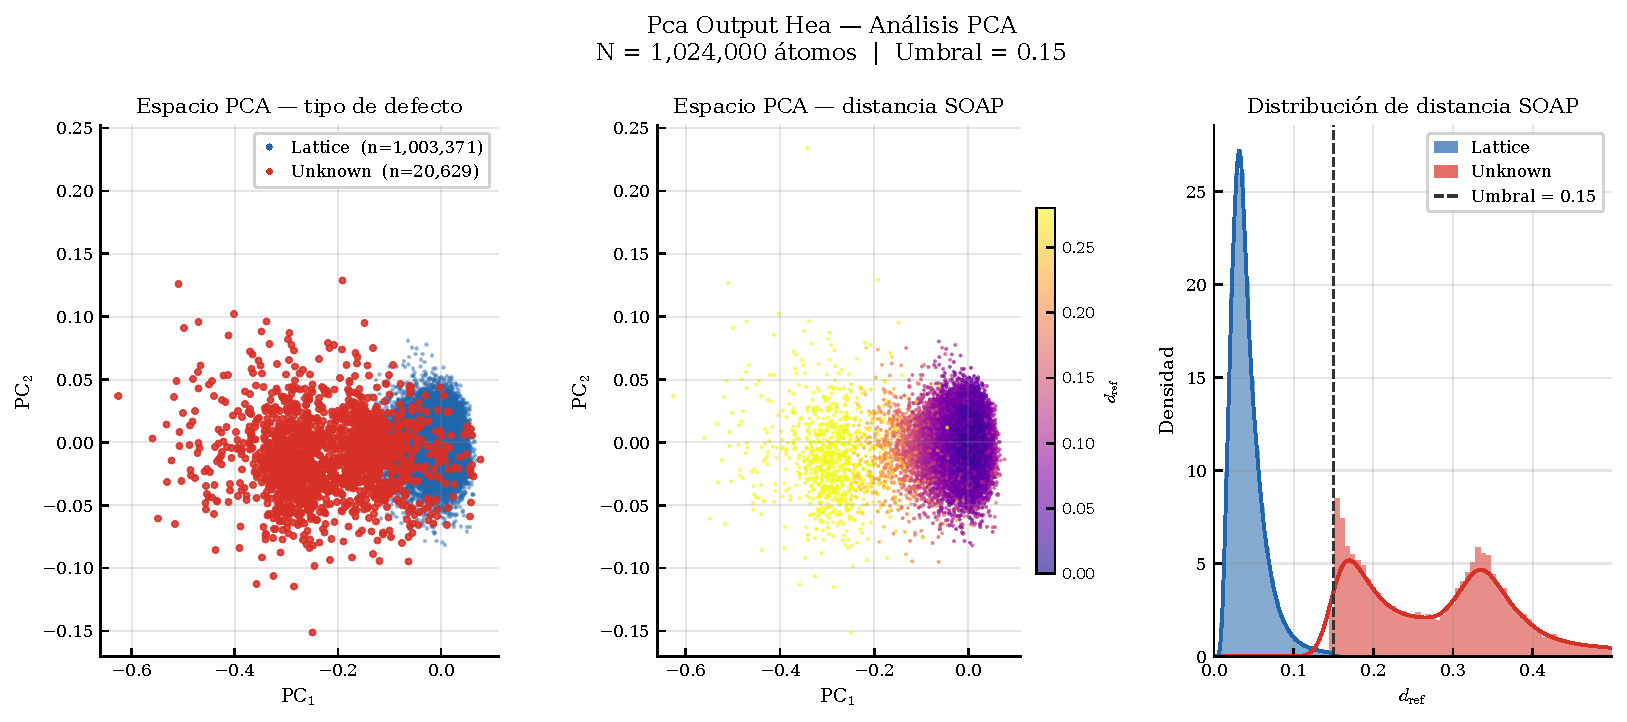
\includegraphics[width=\textwidth]{pca_output_hea_pca}
  \caption{Principal Component Analysis of the 450-dimensional SOAP descriptor
    space for the FeNiCrCoCu HEA.
    \textbf{Left:} Scatter plot of PC$_1$ vs.\ PC$_2$ coloured by
    defect type. The Lattice population forms a dense cluster, while the
    Unknown atoms ($n = 20{,}629$) are dispersed in the peripheral region.
    \textbf{Centre:} Same projection coloured by the SOAP distance
    $d^i$, showing a smooth gradient from lattice to defect environments.
    \textbf{Right:} Distance distribution $d^i$ for both classes, confirming
    the bimodal character already visible in Fig.~\ref{fig:hist}.}
  \label{fig:pca}
\end{figure}

\subsection{Grid-Based Vacancy Mapping}

Figure~\ref{fig:vacancies} shows the spatial distribution of the
$252$ vacancy grid points identified by the grid-based method
(Eq.~\ref{eq:grid}). The three orthogonal projections (XY, XZ, YZ) and
the one-dimensional density profiles reveal that the vacancies are
concentrated in a narrow cylindrical region consistent with the thermal
spike track, in agreement with the SOAP spatial maps in
Fig.~\ref{fig:overview}. The density profiles along each axis allow
quantitative estimation of the track extent: the damaged region spans
approximately $[20, 45]$\,\AA\ in both $x$ and $y$, and extends over
the full $z$ range of the periodic box.

\begin{figure}[H]
  \centering
  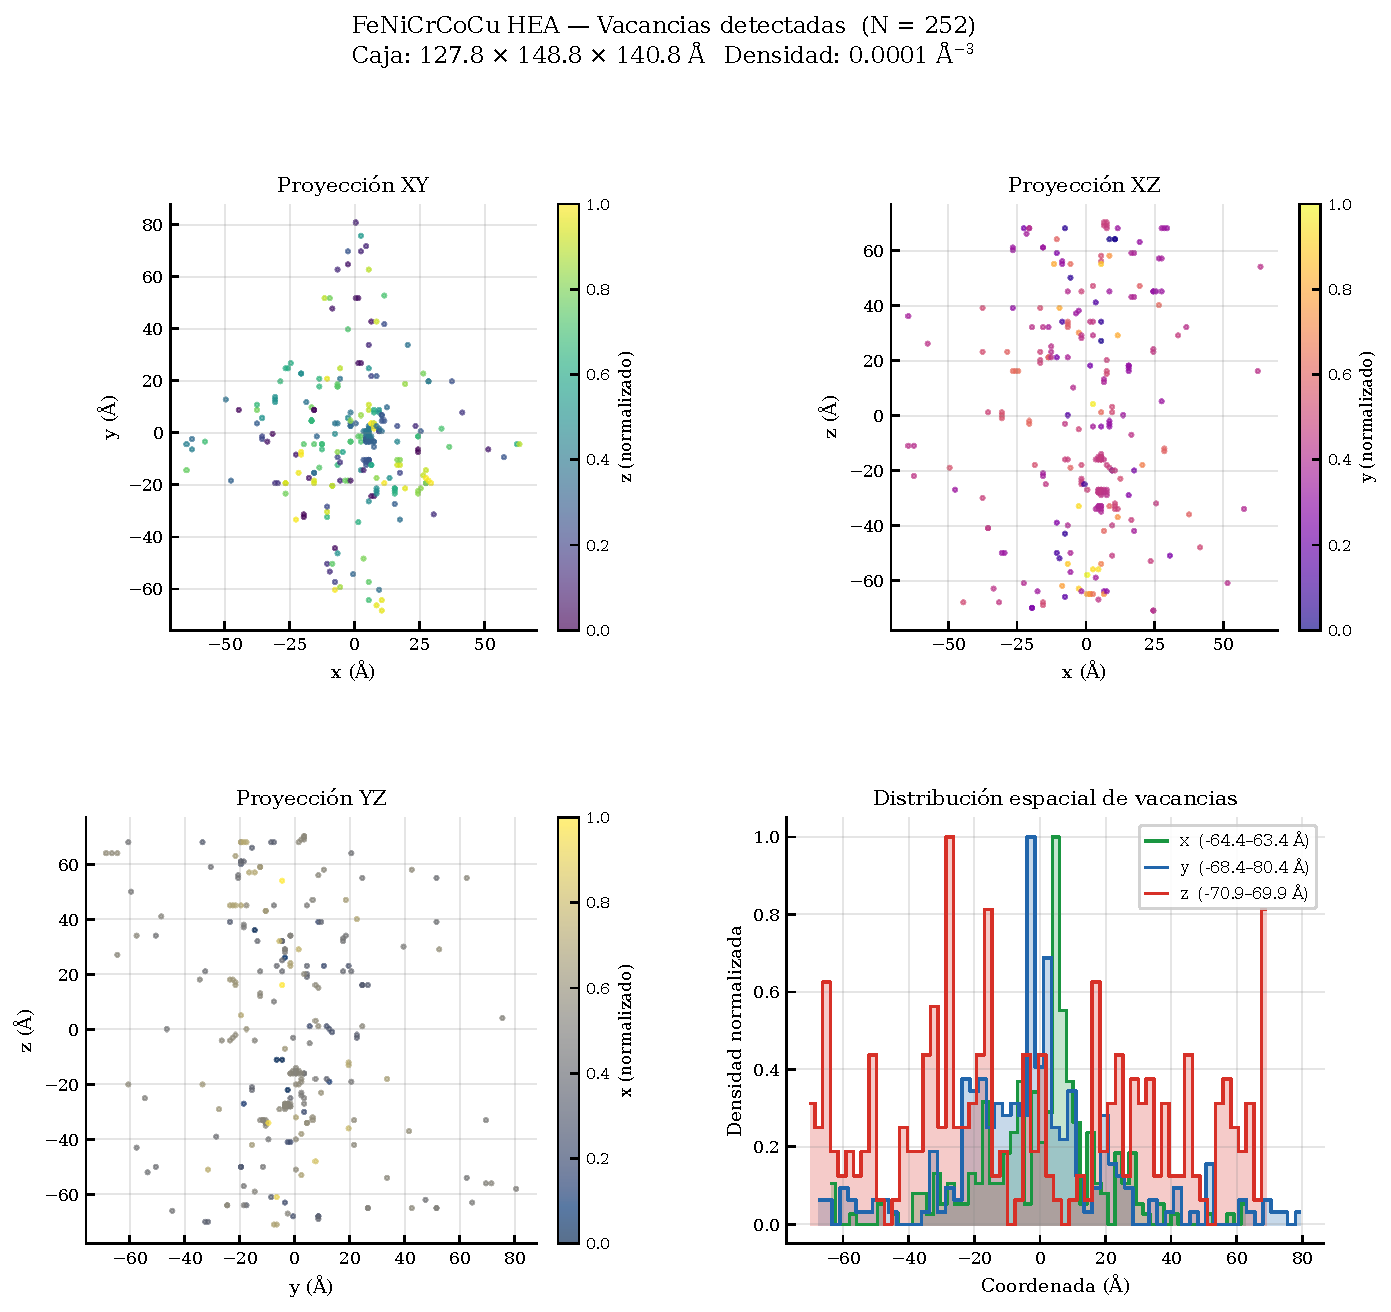
\includegraphics[width=\textwidth]{vacancies_output_hea_vacancies}
  \caption{Spatial distribution of the $252$ vacancy grid points detected
    by the grid-based method (Eq.~\ref{eq:grid}, $d_{\mathrm{vac}} = 2.0$\,\AA)
    in the FeNiCrCoCu HEA after thermal-spike damage.
    \textbf{Top left / Top right / Bottom left:} XY, XZ, and YZ projections
    coloured by the normalised third coordinate, providing depth information.
    \textbf{Bottom right:} Normalised 1-D density profiles along $x$ (green),
    $y$ (blue), and $z$ (red), quantifying the spatial extent of the
    vacancy-rich zone.}
  \label{fig:vacancies}
\end{figure}

\subsection{Comparison of Methods}

Table~\ref{tab:comparison} summarises the defect counts obtained by each
method. The WS method provides an exact count of Frenkel pairs but requires
a reference lattice and fails at high temperature due to thermal displacements.
The SOAP classifier identifies a much larger set of distorted atoms,
capturing both classical point defects and extended defect structures
(e.g.\ stacking faults, amorphous pockets) that WS cannot resolve. The
grid-based vacancy count ($252$) is substantially lower than the WS vacancy
count ($3{,}867$) because it detects only macroscopic voids rather than
individual vacant lattice sites.

\begin{table}[H]
  \centering
  \caption{Defect statistics obtained by the three characterisation methods.}
  \label{tab:comparison}
  \begin{tabular}{lccc}
    \toprule
    Method & Vacancies & Interstitials & Distorted atoms \\
    \midrule
    Wigner--Seitz (OVITO) & $3{,}867$ & $3{,}669$ & --- \\
    SOAP classifier ($d^i \geq 0.15$) & --- & --- & $20{,}629$ \\
    Grid-based ($d_{\mathrm{vac}} = 2.0$\,\AA) & $252$ & --- & --- \\
    \bottomrule
  \end{tabular}
\end{table}

% ─────────────────────────────────────────────────────────────────────────────
\section{Conclusion}
% ─────────────────────────────────────────────────────────────────────────────

Descriptor-based approaches such as SOAP provide a powerful alternative to
classical defect analysis methods, particularly under conditions where
lattice-based approaches fail. The combination of statistical modelling and
local descriptors enables a more complete characterisation of radiation damage
in complex alloys. Applied to a FeNiCrCoCu HEA after a thermal spike, the
SOAP pipeline identifies $20{,}629$ distorted atoms ($2.01\%$ of the system),
reveals the cylindrical morphology of the damage track, and confirms the
physical consistency of the results through PCA-based descriptor-space
analysis.

\section*{Acknowledgments}

[COMPLETAR]

\begin{thebibliography}{99}

\bibitem{Was2017}
G. S. Was, \textit{Fundamentals of Radiation Materials Science},
Springer, 2nd ed.\ (2017).

\bibitem{Zinkle2009}
S. J. Zinkle and G. S. Was,
\textit{Materials challenges in nuclear energy},
Acta Materialia \textbf{61}, 735 (2013).

\bibitem{Yeh2004}
J.-W. Yeh et al.,
\textit{Nanostructured high-entropy alloys with multiple principal elements},
Advanced Engineering Materials \textbf{6}, 299 (2004).

\bibitem{Cantor2004}
B. Cantor et al.,
\textit{Microstructural development in equiatomic multicomponent alloys},
Materials Science and Engineering A \textbf{375--377}, 213 (2004).

\bibitem{Zhang2015radiation}
Y. Zhang et al.,
\textit{Radiation damage in nanostructured materials},
Progress in Materials Science \textbf{96}, 217 (2018).

\bibitem{Granberg2016}
F. Granberg et al.,
\textit{Mechanism of radiation damage reduction in equiatomic multicomponent
single-phase alloys},
Physical Review Letters \textbf{116}, 135504 (2016).

\bibitem{Bartok2013}
A. P. Bartók, R. Kondor, and G. Csányi,
\textit{On representing chemical environments},
Physical Review B \textbf{87}, 184115 (2013).

\end{thebibliography}

\end{document}
